% Research theme figure: Turbulence Modeling
% (energy cascade -> Kolmogorov spectrum -> resolved vs modelled scales).
% Same canvas, fonts and palette as the other research figures; shown in greyscale
% on the site, colour on hover.
% Build (from this folder):
%   latex turbulence.tex
%   dvisvgm --no-fonts --bbox=papersize -o ../turbulence.svg turbulence.dvi
\def\pgfsysdriver{pgfsys-dvisvgm.def}
\documentclass[tikz,border=0pt]{standalone}
\usetikzlibrary{arrows.meta}
\renewcommand{\familydefault}{\sfdefault}

% --- palette (shared with the other research figures) ------------------------
\definecolor{ink}{HTML}{1A1A1A}
\definecolor{frame}{HTML}{4D4D4D}
\definecolor{steel}{HTML}{245A94}
\definecolor{sky}{HTML}{6E9FD2}
\definecolor{mist}{HTML}{D3E3F3}
\definecolor{amber}{HTML}{C8702A}
\definecolor{sand}{HTML}{F0CFA8}

\begin{document}
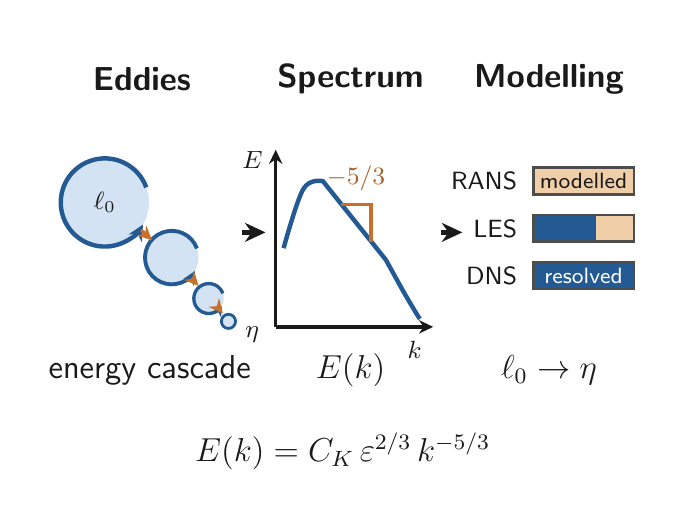
\begin{tikzpicture}[
    line width=1.6pt, >={Stealth[length=2.6mm,width=2.4mm]},
    small arrow/.style={-{Stealth[length=1.8mm,width=1.7mm]}, line width=1.2pt},
    color=ink,
    title/.style={font=\large\bfseries, text=ink},
    lab/.style={font=\large, text=ink}]
  % fixed 8 cm x 6 cm canvas
  \path[use as bounding box] (0,0) rectangle (8,6);

  % ================= 1) energy cascade: big eddies feed smaller ones =================
  \node[title] at (1.45,5.35) {Eddies};
  % eddy: filled disc + rotating arc with arrow head
  \foreach \x/\y/\r/\c in {0.98/3.78/0.56/mist, 1.83/3.08/0.34/mist, 2.30/2.56/0.19/mist, 2.55/2.27/0.09/mist} {
    \fill[\c] (\x,\y) circle (\r);
  }
  \draw[steel, line width=1.6pt, -{Stealth[length=2.0mm,width=1.9mm]}]
    (0.98,3.78) ++(20:0.56) arc[start angle=20, end angle=330, radius=0.56];
  \draw[steel, line width=1.4pt, -{Stealth[length=1.7mm,width=1.6mm]}]
    (1.83,3.08) ++(20:0.34) arc[start angle=20, end angle=330, radius=0.34];
  \draw[steel, line width=1.2pt, -{Stealth[length=1.3mm,width=1.3mm]}]
    (2.30,2.56) ++(20:0.19) arc[start angle=20, end angle=330, radius=0.19];
  \draw[steel, line width=1.0pt] (2.55,2.27) circle (0.09);
  % energy transfer down the scales
  \draw[amber, small arrow] (1.44,3.43) -- (1.58,3.30);
  \draw[amber, small arrow] (2.08,2.82) -- (2.17,2.72);
  \draw[amber, small arrow] (2.43,2.43) -- (2.48,2.37);
  \node[font=\small] at (0.98,3.78) {$\ell_0$};
  \node[font=\small, anchor=west] at (2.62,2.10) {$\eta$};
  \node[lab] at (1.55,1.65) {energy cascade};

  % ================= 2) Kolmogorov energy spectrum (log-log) =================
  \node[title] at (4.10,5.35) {Spectrum};
  \draw[small arrow] (3.15,2.20) -- (5.15,2.20);
  \draw[small arrow] (3.15,2.20) -- (3.15,4.45);
  \node[font=\small, anchor=north east] at (5.15,2.16) {$k$};
  \node[font=\small, anchor=east] at (3.13,4.32) {$E$};
  % production peak -> inertial range (slope -5/3) -> dissipation
  \draw[steel, line width=1.6pt]
    plot[smooth, tension=0.6] coordinates {(3.25,3.20) (3.50,3.95) (3.75,4.05)}
    -- (4.55,3.05)
    plot[smooth, tension=0.6] coordinates {(4.55,3.05) (4.80,2.60) (4.98,2.30)};
  % slope marker
  \draw[amber, line width=1.1pt] (3.98,3.76) -- (4.36,3.76) -- (4.36,3.28);
  \node[font=\small, text=amber!85!black, anchor=south] at (4.17,3.78) {$-5/3$};
  \node[lab] at (4.10,1.65) {$E(k)$};

  % ================= 3) resolved vs modelled scales =================
  \node[title] at (6.62,5.35) {Modelling};
  % bars run from large scales (left) to small scales (right)
  \foreach \name/\y/\res in {RANS/4.05/0.00, LES/3.45/0.62, DNS/2.85/1.00} {
    \node[font=\small, anchor=east] at (6.36,\y) {\name};
    \fill[sand] (6.42,\y-0.17) rectangle (7.70,\y+0.17);
    \fill[steel] (6.42,\y-0.17) rectangle ({6.42+1.28*\res},\y+0.17);
    \draw[frame, line width=1.0pt] (6.42,\y-0.17) rectangle (7.70,\y+0.17);
  }
  % labels inside the bars act as the legend
  \node[font=\footnotesize, text=ink] at (7.06,4.05) {modelled};
  \node[font=\footnotesize, text=white] at (7.06,2.85) {resolved};
  \node[lab] at (6.62,1.65) {$\ell_0 \rightarrow \eta$};

  % ================= arrows between panels =================
  \draw[->] (2.72,3.40) -- (3.02,3.40);
  \draw[->] (5.25,3.40) -- (5.52,3.40);

  % ================= Kolmogorov law =================
  \node[font=\large, text=ink] at (4.00,0.62) {$E(k) = C_K\,\varepsilon^{2/3}\,k^{-5/3}$};
\end{tikzpicture}
\end{document}
